 \chapter{The ATLAS Detector at the Large Hadron Collider}%
\label{sec:detector}

\begin{figure}[ht]
  \centering
  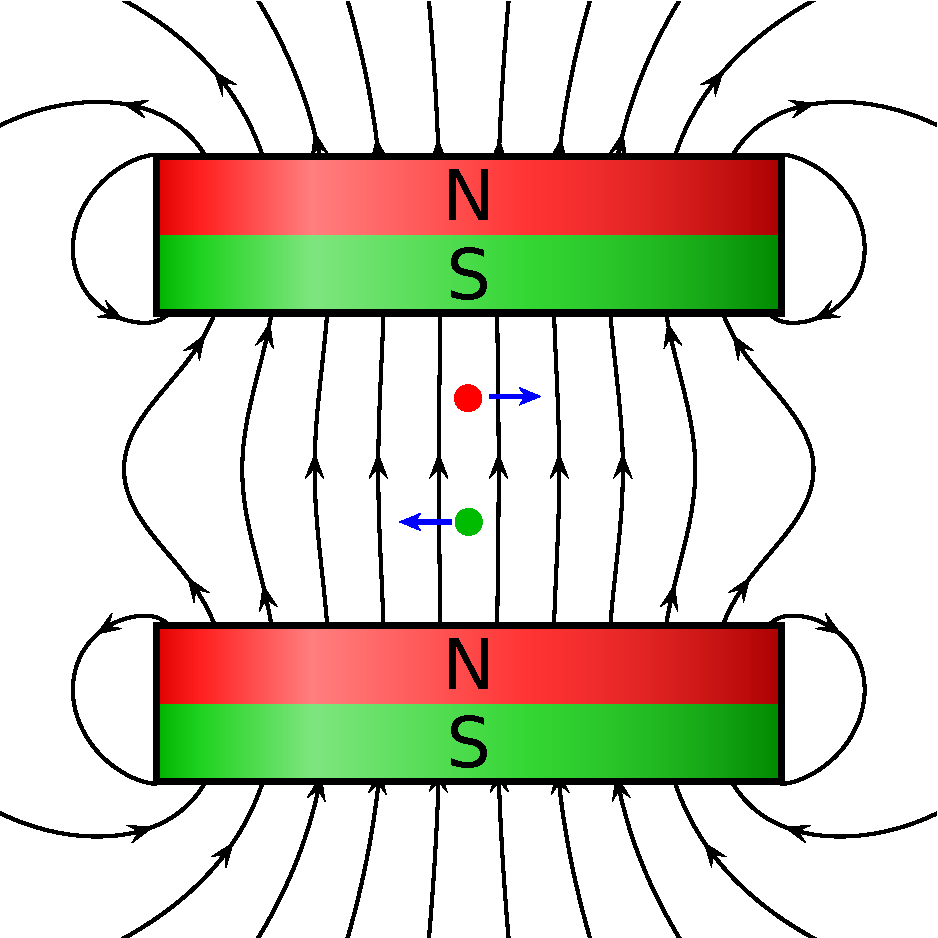
\includegraphics[trim={1cm 1cm 1cm 1cm}, clip, width=.5\textwidth]{uniform_gap}
  \caption[Magnets in a dipole configuration.]{A representation of a pair of
    idealised cylindrical magnets in a dipole configuration. Two positively
    charged particles are shown as circles, the red particle is traveling out of
    the page, the green particle is traveling into the page. The forces
    experienced by each particle due to the magnetic field are shown as blue
    arrows.}
  \label{fig:dipole}
\end{figure}

\begin{figure}[h]
  \centering
  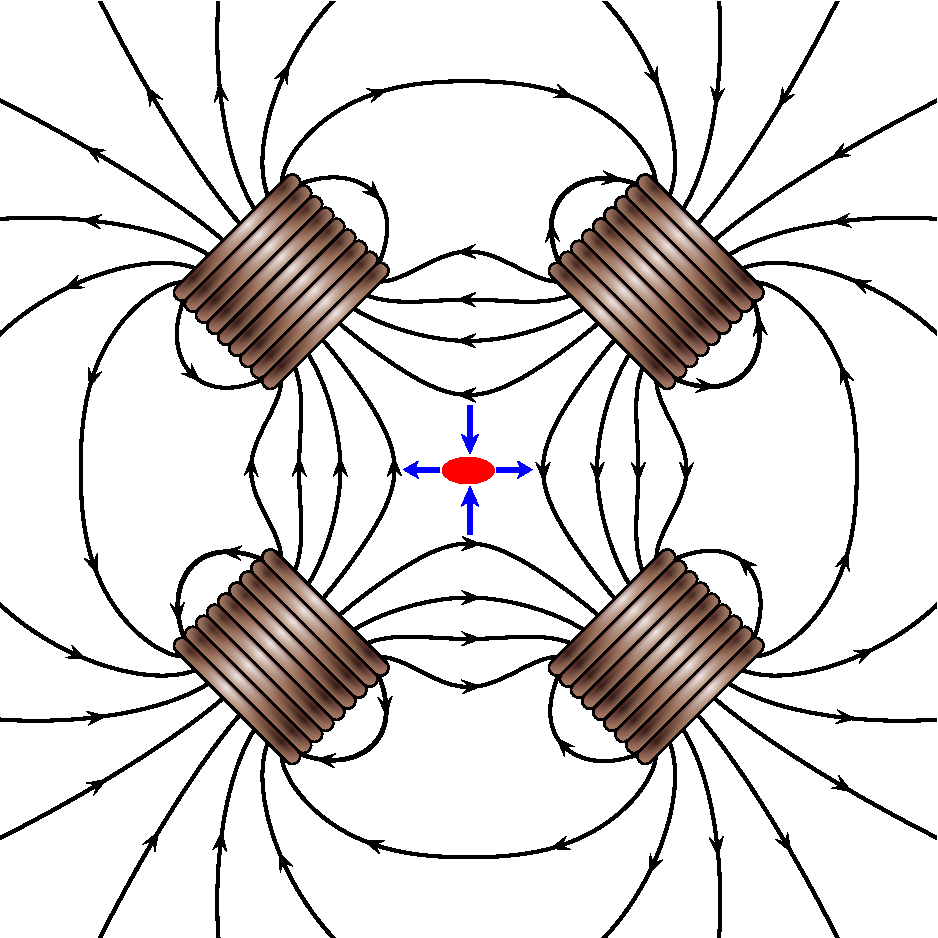
\includegraphics[width=.7\textwidth]{quarupole_with_beamspot}
  \caption{Representation of an idealised set of coil magnets in a quadrupole
    configuration with a proton beamspot shown as a red ellipse. The proton beam
    is drawn coming out of the page (\emph{watch out!}), magnetic field lines
    are drawn in black and the forces acting on each bunch of protons are drawn
    as blue arrows.}
  \label{fig:quadrupole}
\end{figure}

\section{The Large Hadron Collider}%
\label{sec:lhc}%
The Large Hadron Collider (LHC)~\cite{LHC-dr} is a large circular machine
located 100~m underground straddling the Swiss-French border at the European
Organisation for Nuclear Research (CERN). The machine is primarily a proton
collider~\footnote{The LHC also collides other charged particles such as ions of
  lead of xenon.} and is designed so that protons may be accelerated
over to very high energies before being allowed to collide. The diameter of the
LHC is 27~km, it resides in a tunnel which was originally excavated for the
Large Electron-Positron Collider~\cite{LEP} experiment and at the time was the
largest civil engineering project in Europe. Today there are many experiments at
CERN, all with the goal of improving our understanding of a particular area of
physics some of which are marked in figure.~\ref{fig:lhc-acc}. In particular
there are seven experiments that record data from the collisions at the LHC:
ATLAS~\cite{ATLAS-loi}, CMS~\cite{CMS-loi}, LHCb~\cite{lhcb-loi},
ALICE~\cite{ALICE-loi}, MoEDAL~\cite{MoEDAL-loi}, TOTEM~\cite{TOTEM-loi} and
LHCf~\cite{lhcf-loi}.
\begin{figure}[h]
  \centering
  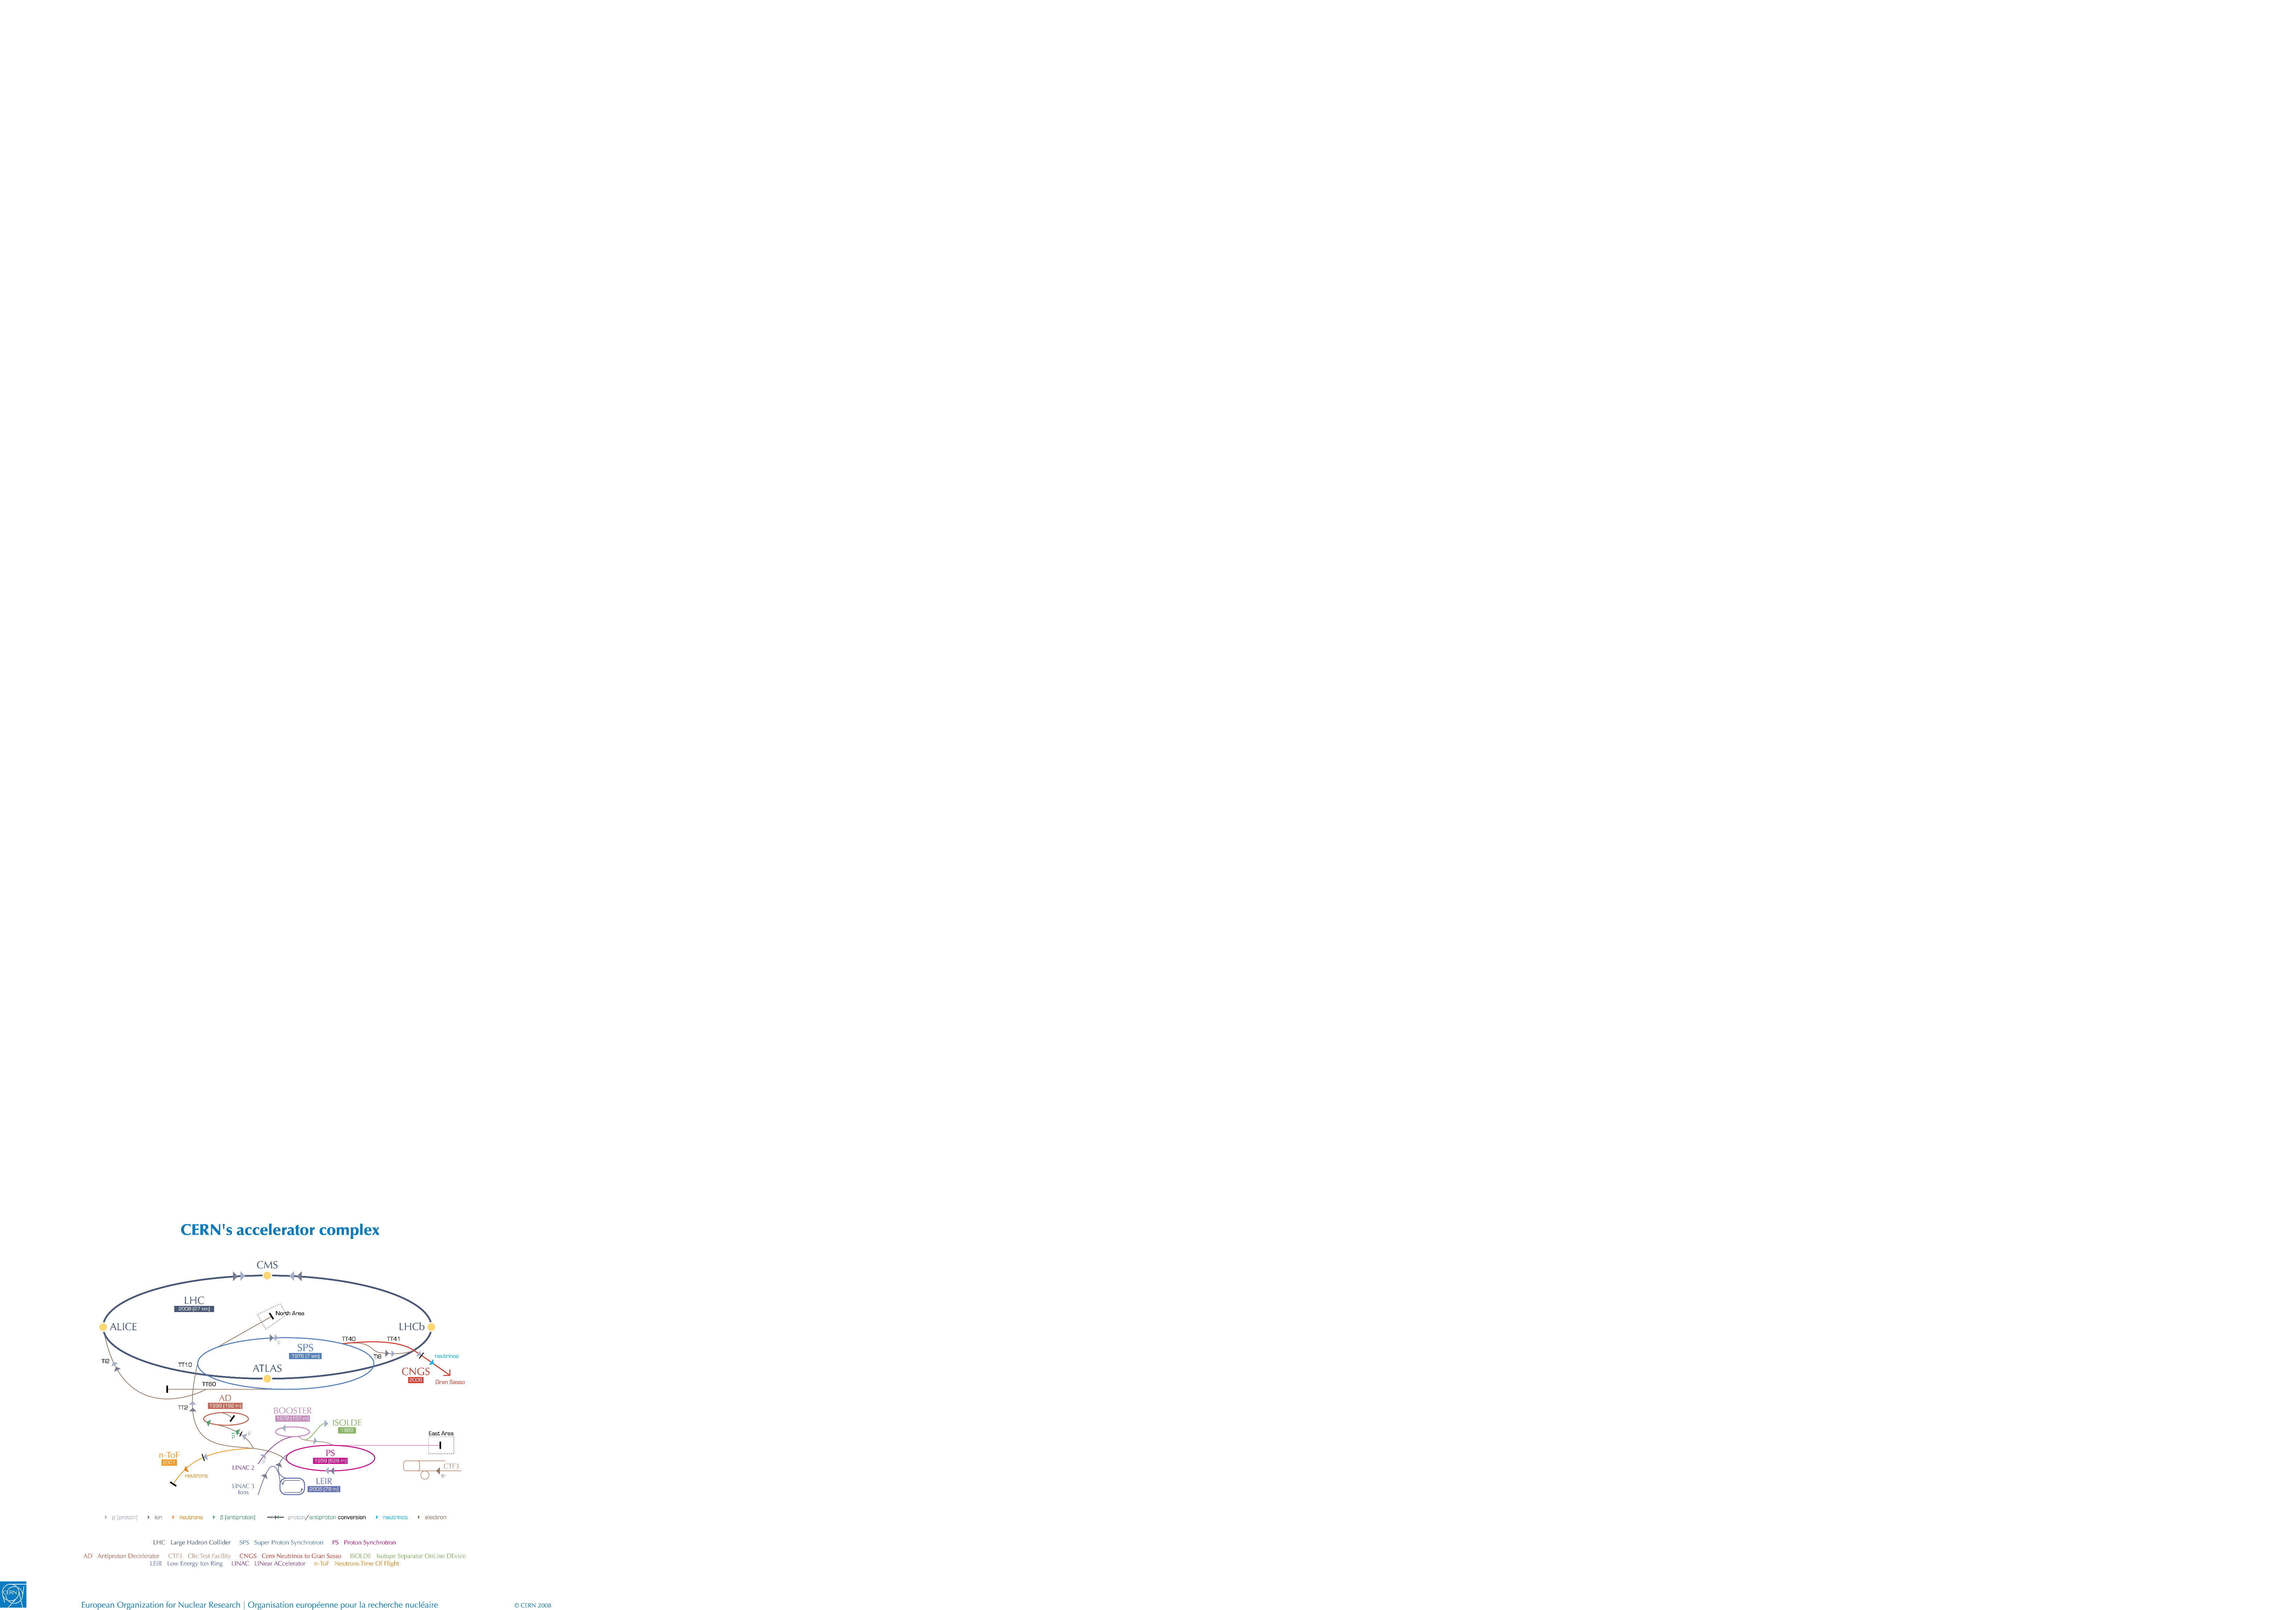
\includegraphics[width=.7\textwidth]{lhc-accelerator}
  \caption[The CERN accelerator complex]{The CERN accelerator
    complex~\cite{LHC-acc-fig}.}%
  \label{fig:lhc-acc}
\end{figure}

The LHC receives protons that have already been accelerated somewhat by the
Super Proton Synchrotron (SPS), another of the accelerators at the CERN
accelerator complex shown in figure~\ref{fig:lhc-acc}. The circular design of
both the LHC and SPS allows protons to be accelerated many times around their
respective rings until their velocity is fast enough for a high energy
collision. The highest energy collisions achieved take place at a centre of mass
energy of $\sqrt{s} = 13 $~TeV, although the design energy of the LHC is
$\sqrt{s} = 14 $~TeV. Despite having not yet reached its design energy the LHC
collides particles with the highest energy of any particle collider in history
and is currently alone at the energy frontier of modern physics. At the time of
writing the LHC is in it's second long shutdown during which maintenance and
upgrades to the LHC and the particle detectors located around its ring take
place. The LHC has completed two runs data taking from collisions, Run 1 took
place from 2009 to 2013, followed  by Run 2
between 2015 and 2018. The period between runs is known as long shutdown 1 (LS1), and
was used to perform maintenance and upgrades. Many analyses from Run 1 have been
published including, most notably the discovery of the Higgs
boson~\cite{DiscoHiggsATLAS, DiscoHiggsCMS}. Some Run 2 analyses have also
published results a highlight of which is LHCb's discovery of charge parity
violation in charm decays~\cite{cp-charm}. Despite these impactful results there
are many more results expected from the LHC experiments as data continues to be
analysed.

The statistical nature of particle physics analyses means that larger datasets
(more recorded collisions) increase the sensitivity of searches and
measurements. Constraints on the number of years the LHC is able to run for mean
that the best way to record more collisions is to collide more particles per
second. A quantity known as the luminosity is often used to describe how much
data is available for an analysis, it is written as
\begin{equation}
  \label{eq:luminosity}
  L = \frac{1}{\sigma}\frac{dN}{dt},
\end{equation}
where $\sigma$ is the interaction cross-section, a volume within which particles
must pass by one another in order to interact, and $N$ is the number of events
recorded in a period of time $t$. For luminosity at the LHC N can be expressed as
\begin{equation}
  \label{eq:lhc-lumi}
  N = n_{bp}n_{1}n_{2}\nu_{r},
\end{equation}
where $n_{bp}$ is the number of colliding bunch pairs, $n_{1}$ and $n_{2}$ are
the number of protons in each beam and $\nu_r$ is the frequency with which the
beams rotate around the LHC's circumference. It is clear that to increase
luminosity any one of these parameters can be increased. The LHC has already
exceeded it's design luminosity providing physicists with more data to analyse
than expected and plans are well underway for the upgrade to a High-Luminosity
LHC (HL-LHC)~\cite{hilumi-tdr}.

\section{The ATLAS Detector}%
\label{sec:atlas}

The ATLAS detector~\cite{ATLAS} resides at a location on the LHC ring called
Point 1, its full name is A Toroidal LHC ApparatuS. A diagram of the detector is
shown in figure~\ref{fig:ATLAS-det}. ATLAS is considered to be a general purpose
particle detector and has a wide physics program including: Higgs boson physics,
top quark physics, searches for Supersymmetry and exotic states, probes of CP
violation in b-quarks and light states and heavy ion physics. The work in this
report is concerned with the measurement of products from proton-proton
collisions. The detector itself is very large in size, spanning a width of 25~m
and a length of 44~m and weighs 7000~tonnes which is comparable to the weight of
the wrought iron content of the Eiffel tower~\cite{Eiffel-weight}.
\begin{figure}[h]
  \centering
  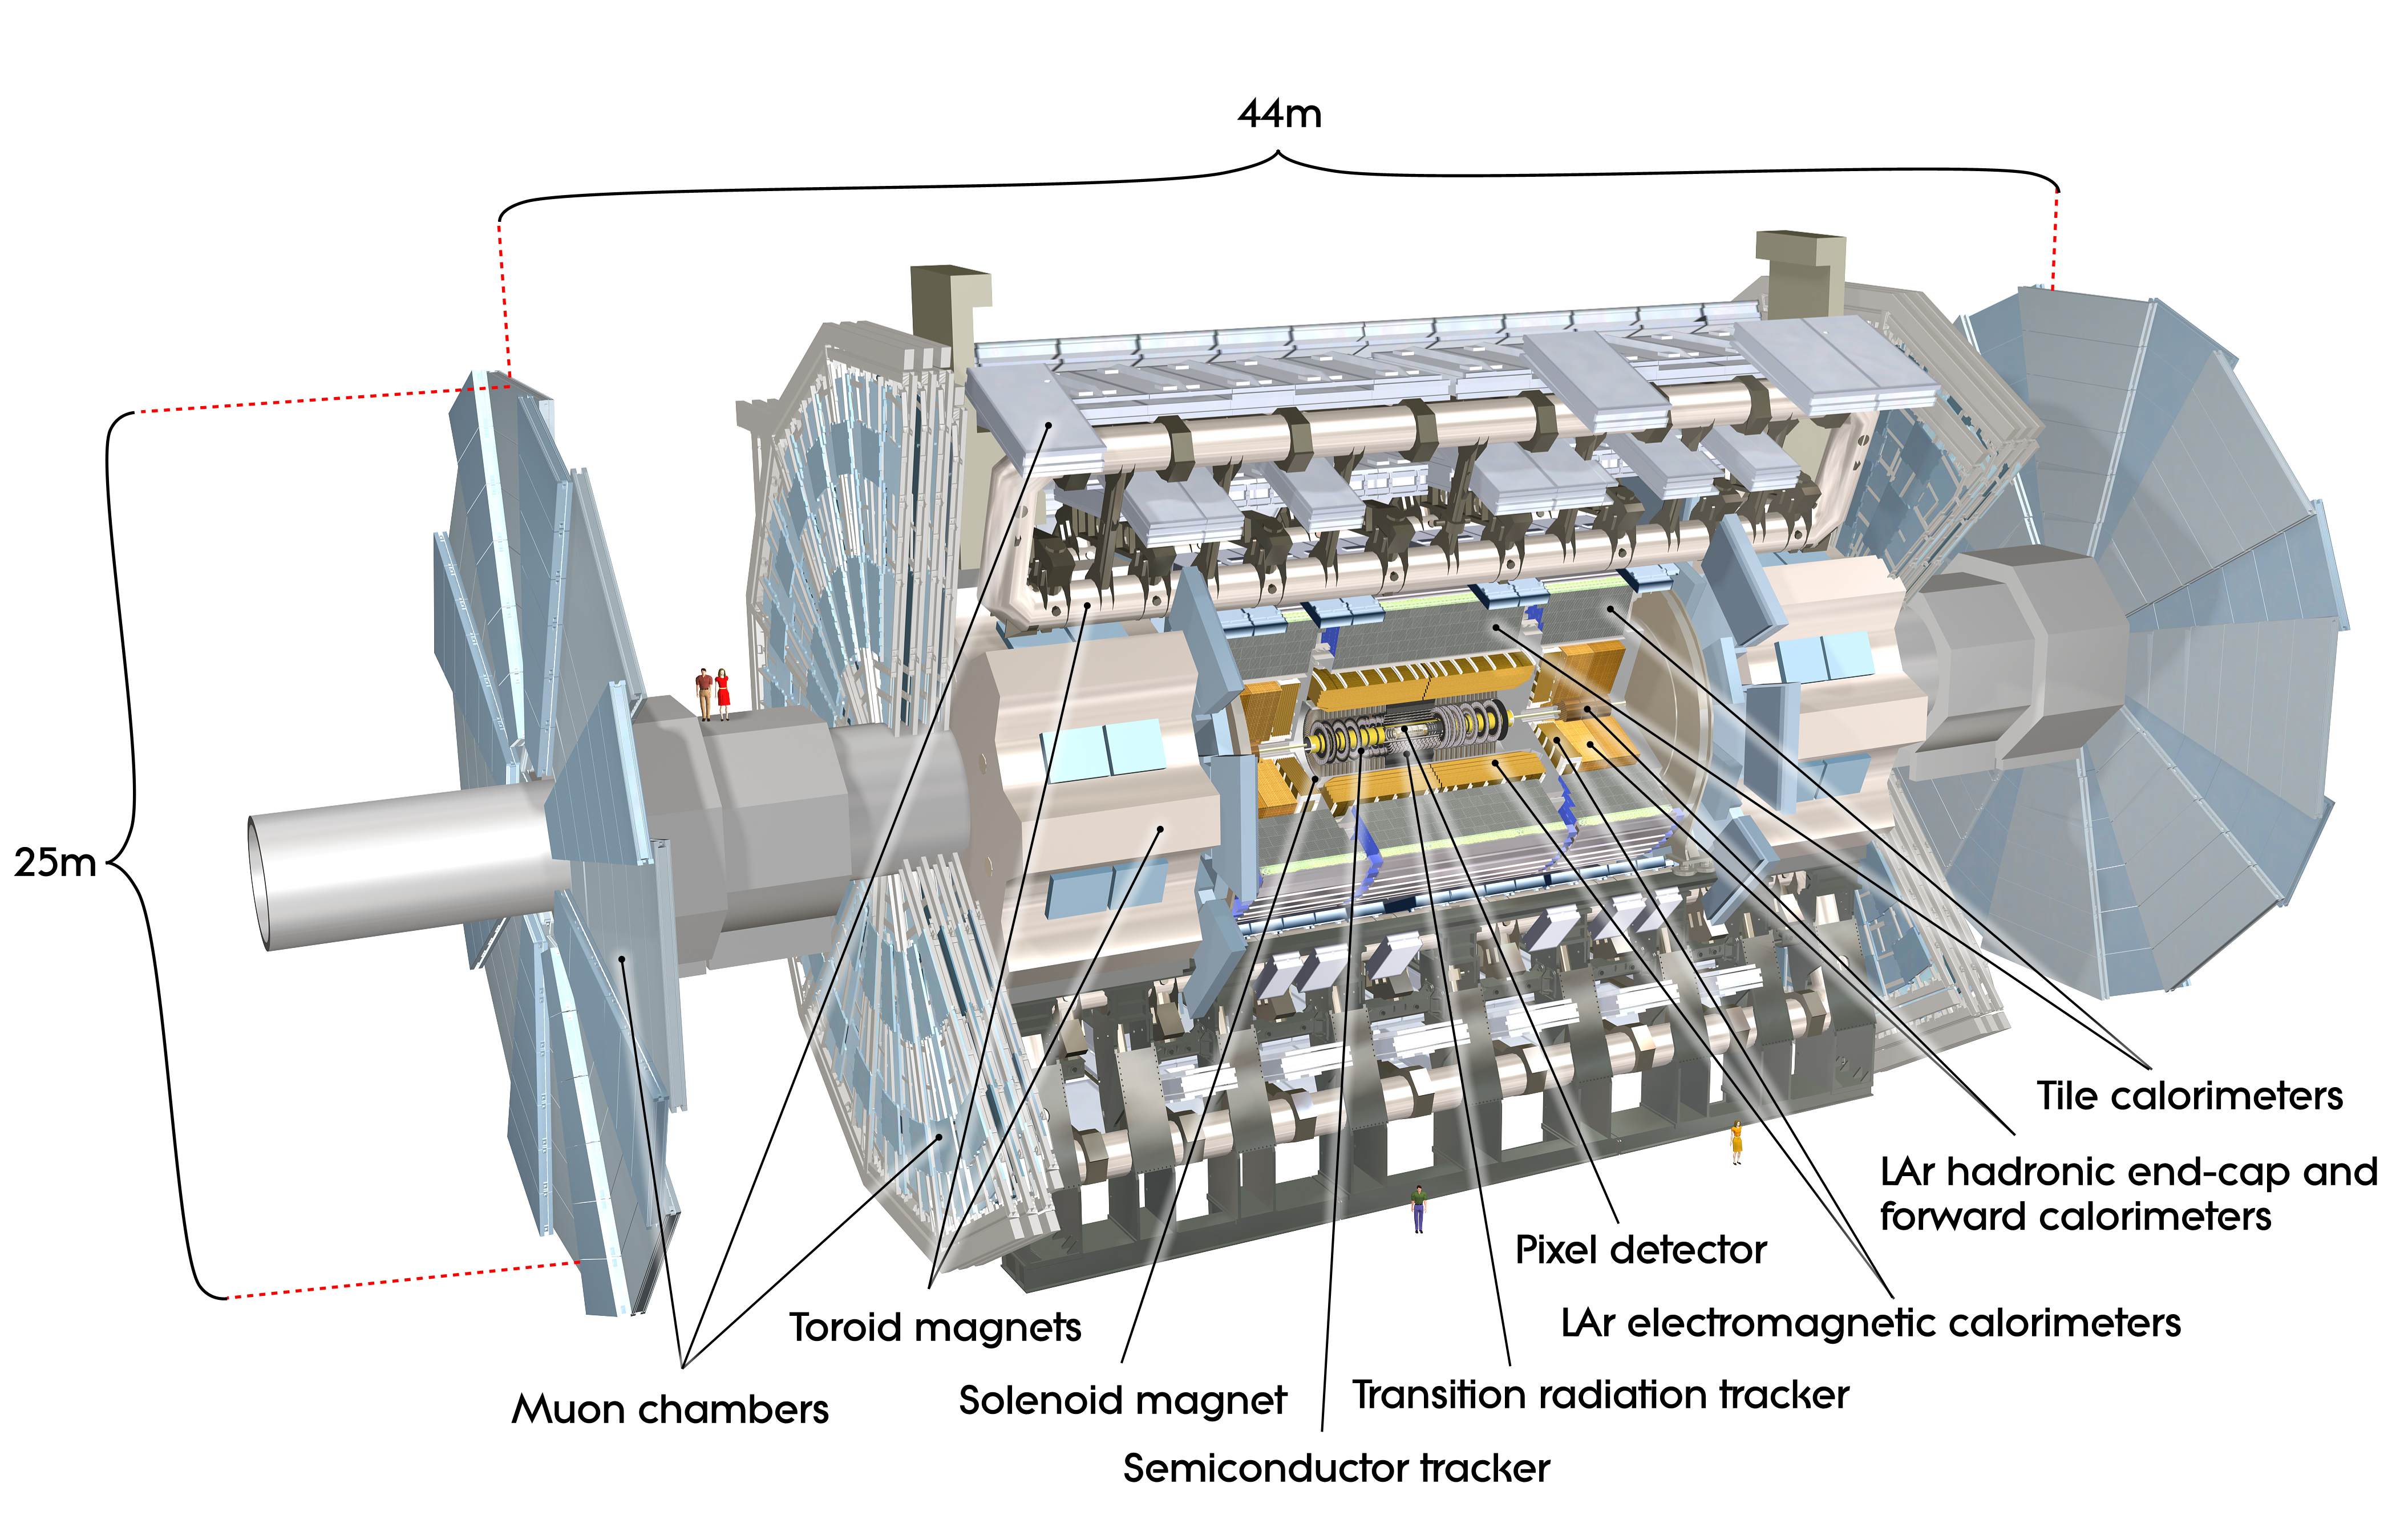
\includegraphics[width=.7\textwidth]{ATLAS-detector}
  \caption[The ATLAS Detector]{Computer generated image of the whole ATLAS
    detector with the major sub detectors labeled~\cite{ATLAS-det-fig}.}%
  \label{fig:ATLAS-det}
\end{figure}


Due to the composite nature of the proton, the decay products of collisions are
extremely numerous. Additionally when two bunches of protons cross there is the
chance that more than one hard scattering event occurs and softer glancing
collisions are also a possibility. The number of hard scattering events in a
given bunch crossing is known as the pile-up of the collision and is often
denoted with the symbol $\mu$. As can be seen by inspecting
equations~\ref{eq:lhc-lumi}~and~\ref{eq:luminosity} increasing the luminosity
will often cause a higher pile-up environment in the detector. High pile-up,
along with the numerous decay products of each collision necessitate the use of
specialised sub-detectors in order to accurately measure the output of
collisions. For certain types of decay product there are different dedicated
sub-systems in ATLAS with the purpose of measuring properties of particles of
that type. At this stage it is sufficient to say that the treatment of
electrically charged particles must be different to those that are electrically
neutral, but this concept will be expanded upon in more detail in the further
sections. It is interesting to note that despite the many charges that are
associated with the forces of nature discussed in chapter~\ref{sec:theory} the
only one that we can directly measure is electric charge.%\footnote{This is true
  %for current human technology, it is not known if future or alien technology
  %can access other charges.}.

The ATLAS sub-systems are located in either the barrel of the detector or one of
the end-caps. These two areas have a different geometry and so the design of a
sub-system in the barrel will differ from the same sub-system in the end-cap.
What follows is a description of the ATLAS sub-systems and their individual
components, for each component more detail will be given about which properties
of which types of particles it is used to measure. These details are based on
the ATLAS technical design report volumes~\cite{ATLAS-TDR-01, ATLAS-TDR-02}
unless another citation is present. Before detailing individual components it is
important to detail certain properties of the detector relevant to all
sub-systems.  The coordinate system used to describe the ATLAS detector is known
as right-handed. Three orthogonal axes $(x, y, z)$ are used to describe the 3D
space of the detector. The x-axis points towards the centre of the LHC ring, the
y-axis points upwards and the z-axis points along the LHC beam pipe y-axis. The
three axes meet at the interaction point which is the nominal position where
bunches cross, located in the centre of the detector. Cylindrical coordinates
$(r, \phi)$ are also often used to describe the physical features of the
detector and phenomena caused by interactions in the detector that shall be
referred to as analysis objects. Their definitions are that $\phi$ is the
azimuthal angle in the x-y plane (transverse) around the beam pipe and $r$ is
the distance from the interaction point. A final quantity used due to its
compatibility with description relativistic objects in the detector is
pseudo-rapidity $\eta = - \ln(\tan(\theta / 2))$ where $\theta$ is the zenith
angle measured from the z-axis.

The grouping of particles into electrically charged or neutral is largely due to
the fact charged particles experience the Lorentz force
\begin{equation}
  \label{eq:lorentz}
  \vec{F} = q(\vec{E} + \vec{v} \times \vec{B}),
\end{equation}
whereas neutral particles have $q=0$, and so they do not. The magnetic field
$\vec{B}$ has the effect of changing the direction of the particles trajectory
only. This is due to the fact that any force $\vec{F}$ resulting from the cross
product of two vectors, in this case the field vector and the velocity $\vec{v}$,
much act in a perpendicular to the two crossed vectors and thus perpendicular to
the direction of the motion (the direction of velocity). Similarly the electric
field term $\vec{E}$ has the effect that the particle is accelerated in the
direction (or opposite in the case of a negative particle) of the field lines.
The consequence of this is that in a known magnetic field the velocity of a
particle can be calculated by measuring the radius of curvature of its
trajectory. In order to exploit these properties of charged particles a large
portion of the ATLAS detector is immersed in magnetic fields created by the
magnet systems. There are four magnet systems in ATLAS the solenoid, the barrel
toroid, and two end-cap toroids. The solenoid surrounds the inner detector
whilst the toroid systems surround the muon chambers.
Figure~\ref{fig:ATLAS-magnets} shows a heat map of the magnetic field strengths
within ATLAS, the image is from an article detailing the superconducting magnet
system~\cite{ATLAS-magnets}. The magnet systems store a total energy of 1.6~GJ
and produce fields of a combined volume of approximately
$12\times 10^4$~m$^3$.
\begin{figure}[h]
  \centering
  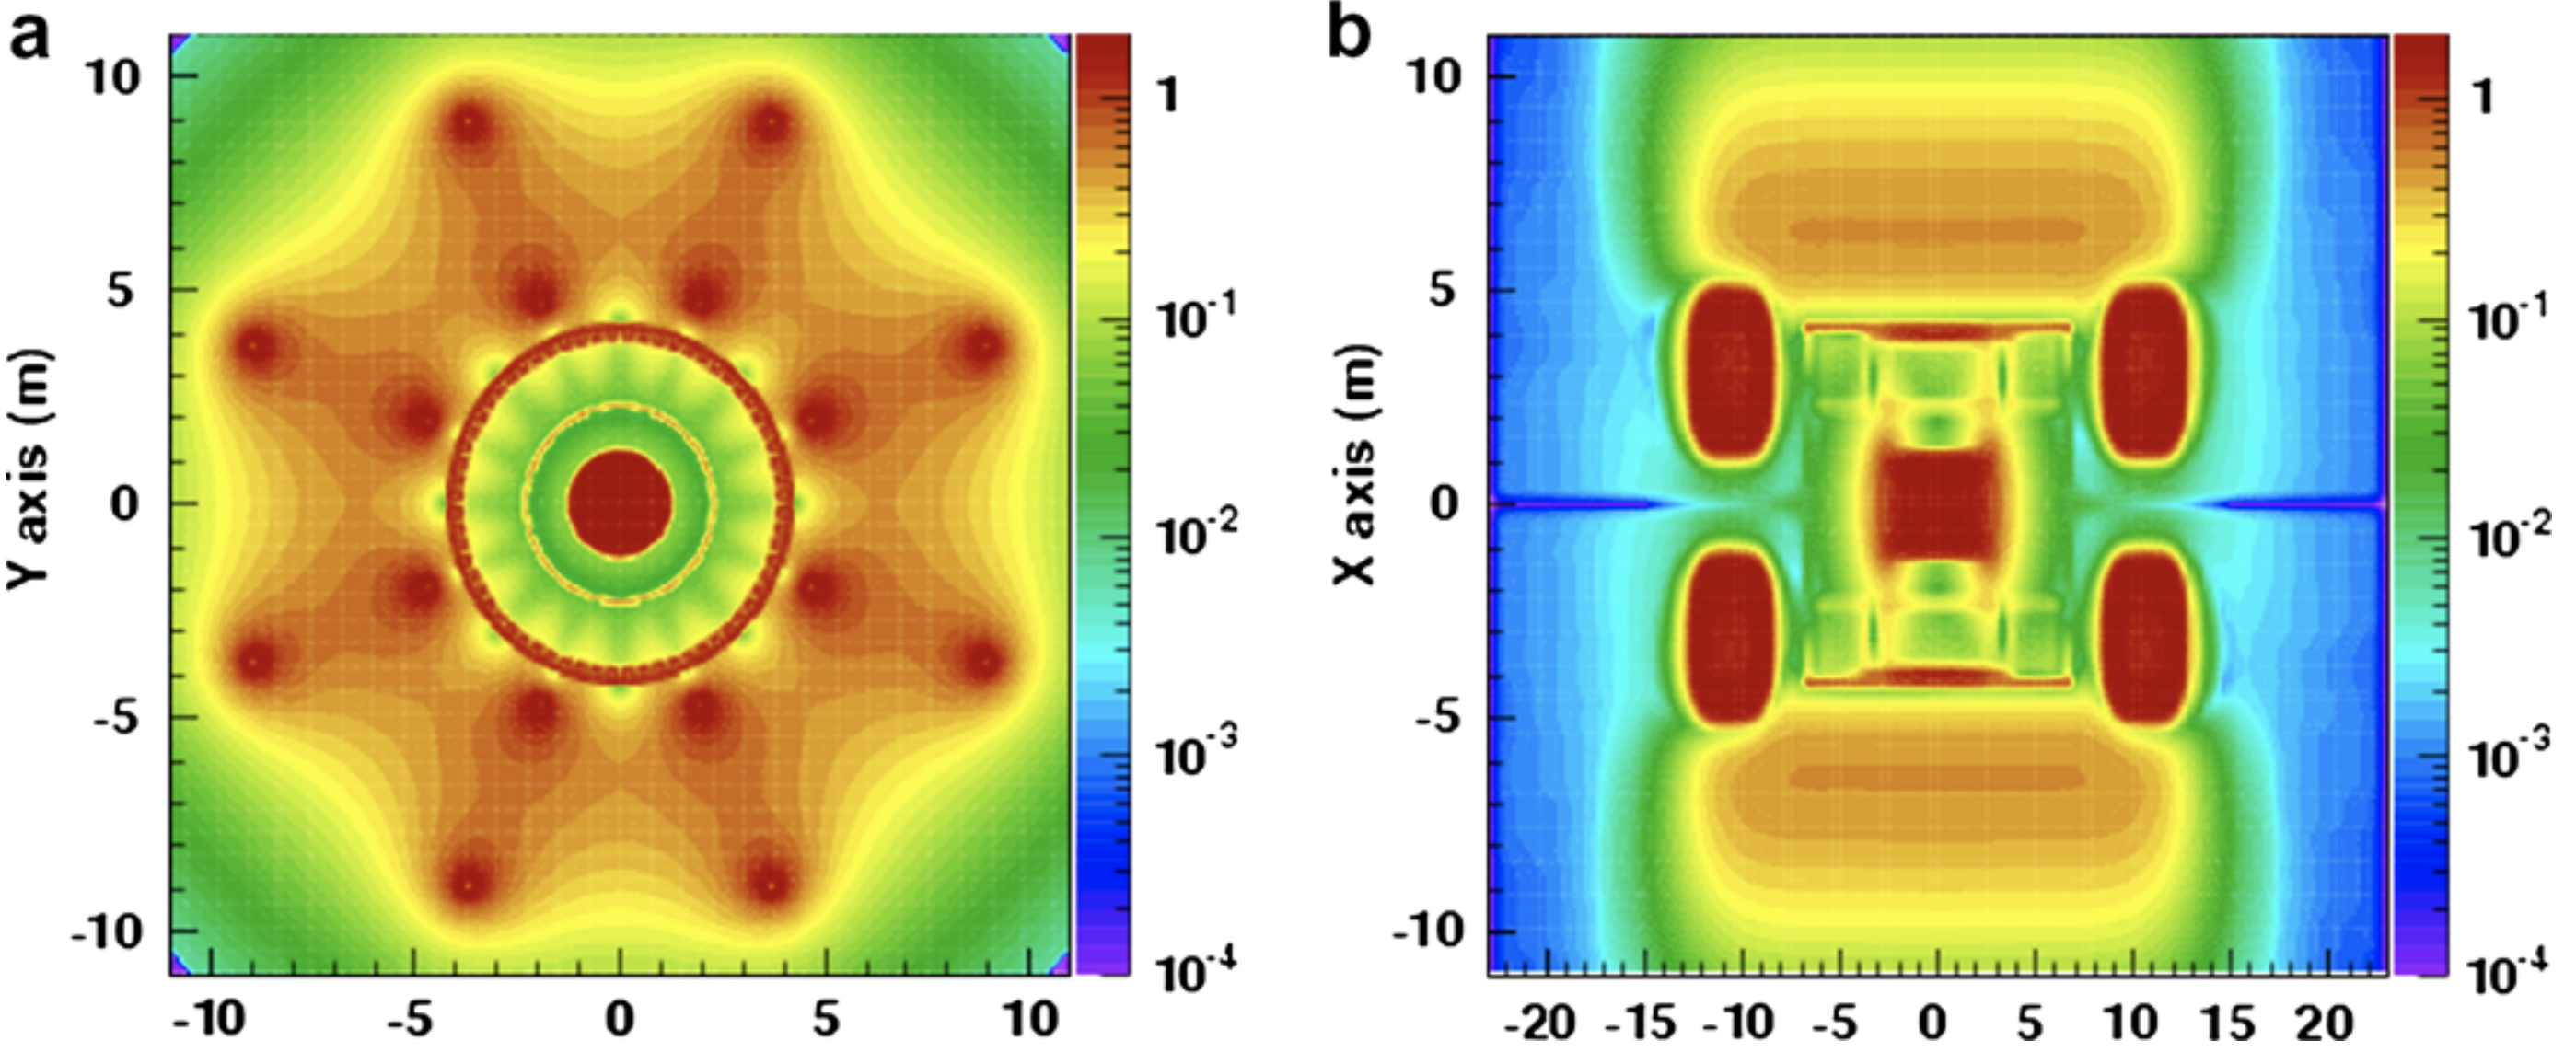
\includegraphics[width=.7\textwidth]{ATLAS-magnet}
  \caption[ATLAS magnetic field]{ATLAS magnetic field profile, showing a
    transverse cross-section in the centre of the detector (a), and a
    longitudinal section (b)~\cite{ATLAS-magnets}.}%
  \label{fig:ATLAS-magnets}
\end{figure}

\subsection{Inner Detector}%
\label{sec:id}

The Inner Detector (ID) is comprised of pixel detectors, the semiconductor
tracker (SCT) and a transition radiation tracker (TRT) as seen in
figure~\ref{fig:ATLAS-inner-det}. It covers a volume corresponding with the
total $\phi$ angle. In relation to $\eta$ the pixel detectors and SCT cover the
range $|\eta|~<~2.5$ and the TRT covers $|\eta|~<~2.0$. Being the innermost
sub-detector of ATLAS the primary goals of the ID are to reconstruct the
locations of the origin of interactions (known as the interaction vertex), and
to track the propagation of charged particles through the detector. This is
achieved by measuring a sequence of hits for each charged particle that
propagates through its material, upon which reconstruction algorithms can be
applied, known as track finding algorithms. From this sequence of hits
interaction vertices can also be reconstructed, the vertex which comes from the
highest energy collision in a given event is known as the primary vertex.
Information from the tracker is used to match activity in outer regions of the
detector to an interaction vertex. Each reconstructed track will have a momentum
assigned to it, which is calculated using equation~\ref{eq:lorentz}. The
magnetic field that the ID is immersed in is produced by the solenoid magnet
system. The system is made of a single layer coil with an inner diameter of
2.46~m  and produces 2~T field in the axial direction with respect to the
beam-pipe.
\begin{figure}[h]
  \centering
  \includegraphics[width=.7\textwidth]{Inner-detector}
  \caption[ATLAS inner detector]{Computer generated image of the ATLAS inner
    detector~\cite{ATLAS-inner-det}.}%
  \label{fig:ATLAS-inner-det}
\end{figure}

\subsubsection{Pixel Detectors}

There are four layers of pixel detectors that are the closest components of the
ID to the beam-pipe. The design originally had three layers, each 250~$\mu$m
thick with 50~$\mu$m by 250~$\mu$m pixels, of oxygen doped n-type silicon
crystals. During LS1 a fourth layer, closest to the beam-pipe (which was also
replaced for a smaller radius version) was added. This layer is known as the
insertable B-layer (IBL)~\cite{IBL-TDR}, the motivation for its addition was to
counteract degradation of original performance of the ID due to irreversible
damage by radiation. As well as the inclusion of the IBL, performance degradation
is mitigated by increasing the bias voltage across the pixels from 100~V (their
starting voltage) to up to 600~V. Additionally the IBL being closer to the
beam-pipe allows for interaction vertices to be measured more precisely. The
need for better reconstruction of vertices is motivated by their role in the
performance of algorithms that classify jets of activity in the detector that
are initiated by B-hadrons, this is where the IBL gets its name. There are no
pixel detectors in the end-caps.

\subsubsection{Semiconductor Tracker}

Next closest to the beam-pipe are the semiconductor trackers. Similarly to the pixel
detectors the semiconductor trackers are also made of silicon. In contrast to
the n-type silicon of the pixels, the semiconductor trackers use p-in-n type
technology. The semiconductor modules are comprised of two back to back silicon
wafers that are offset by a small angle in order to improve coverage. Each wafer
has a series of strips of p-in-type material covered in a metalised layer, the
strips are separated by a distance of 80~$\mu$m. The strips have a bias voltage
applied and on the wafers the necessary electronics are mounted for readout as
seen in figure~\ref{fig:strip-module}.
\begin{figure}[h]
  \centering
  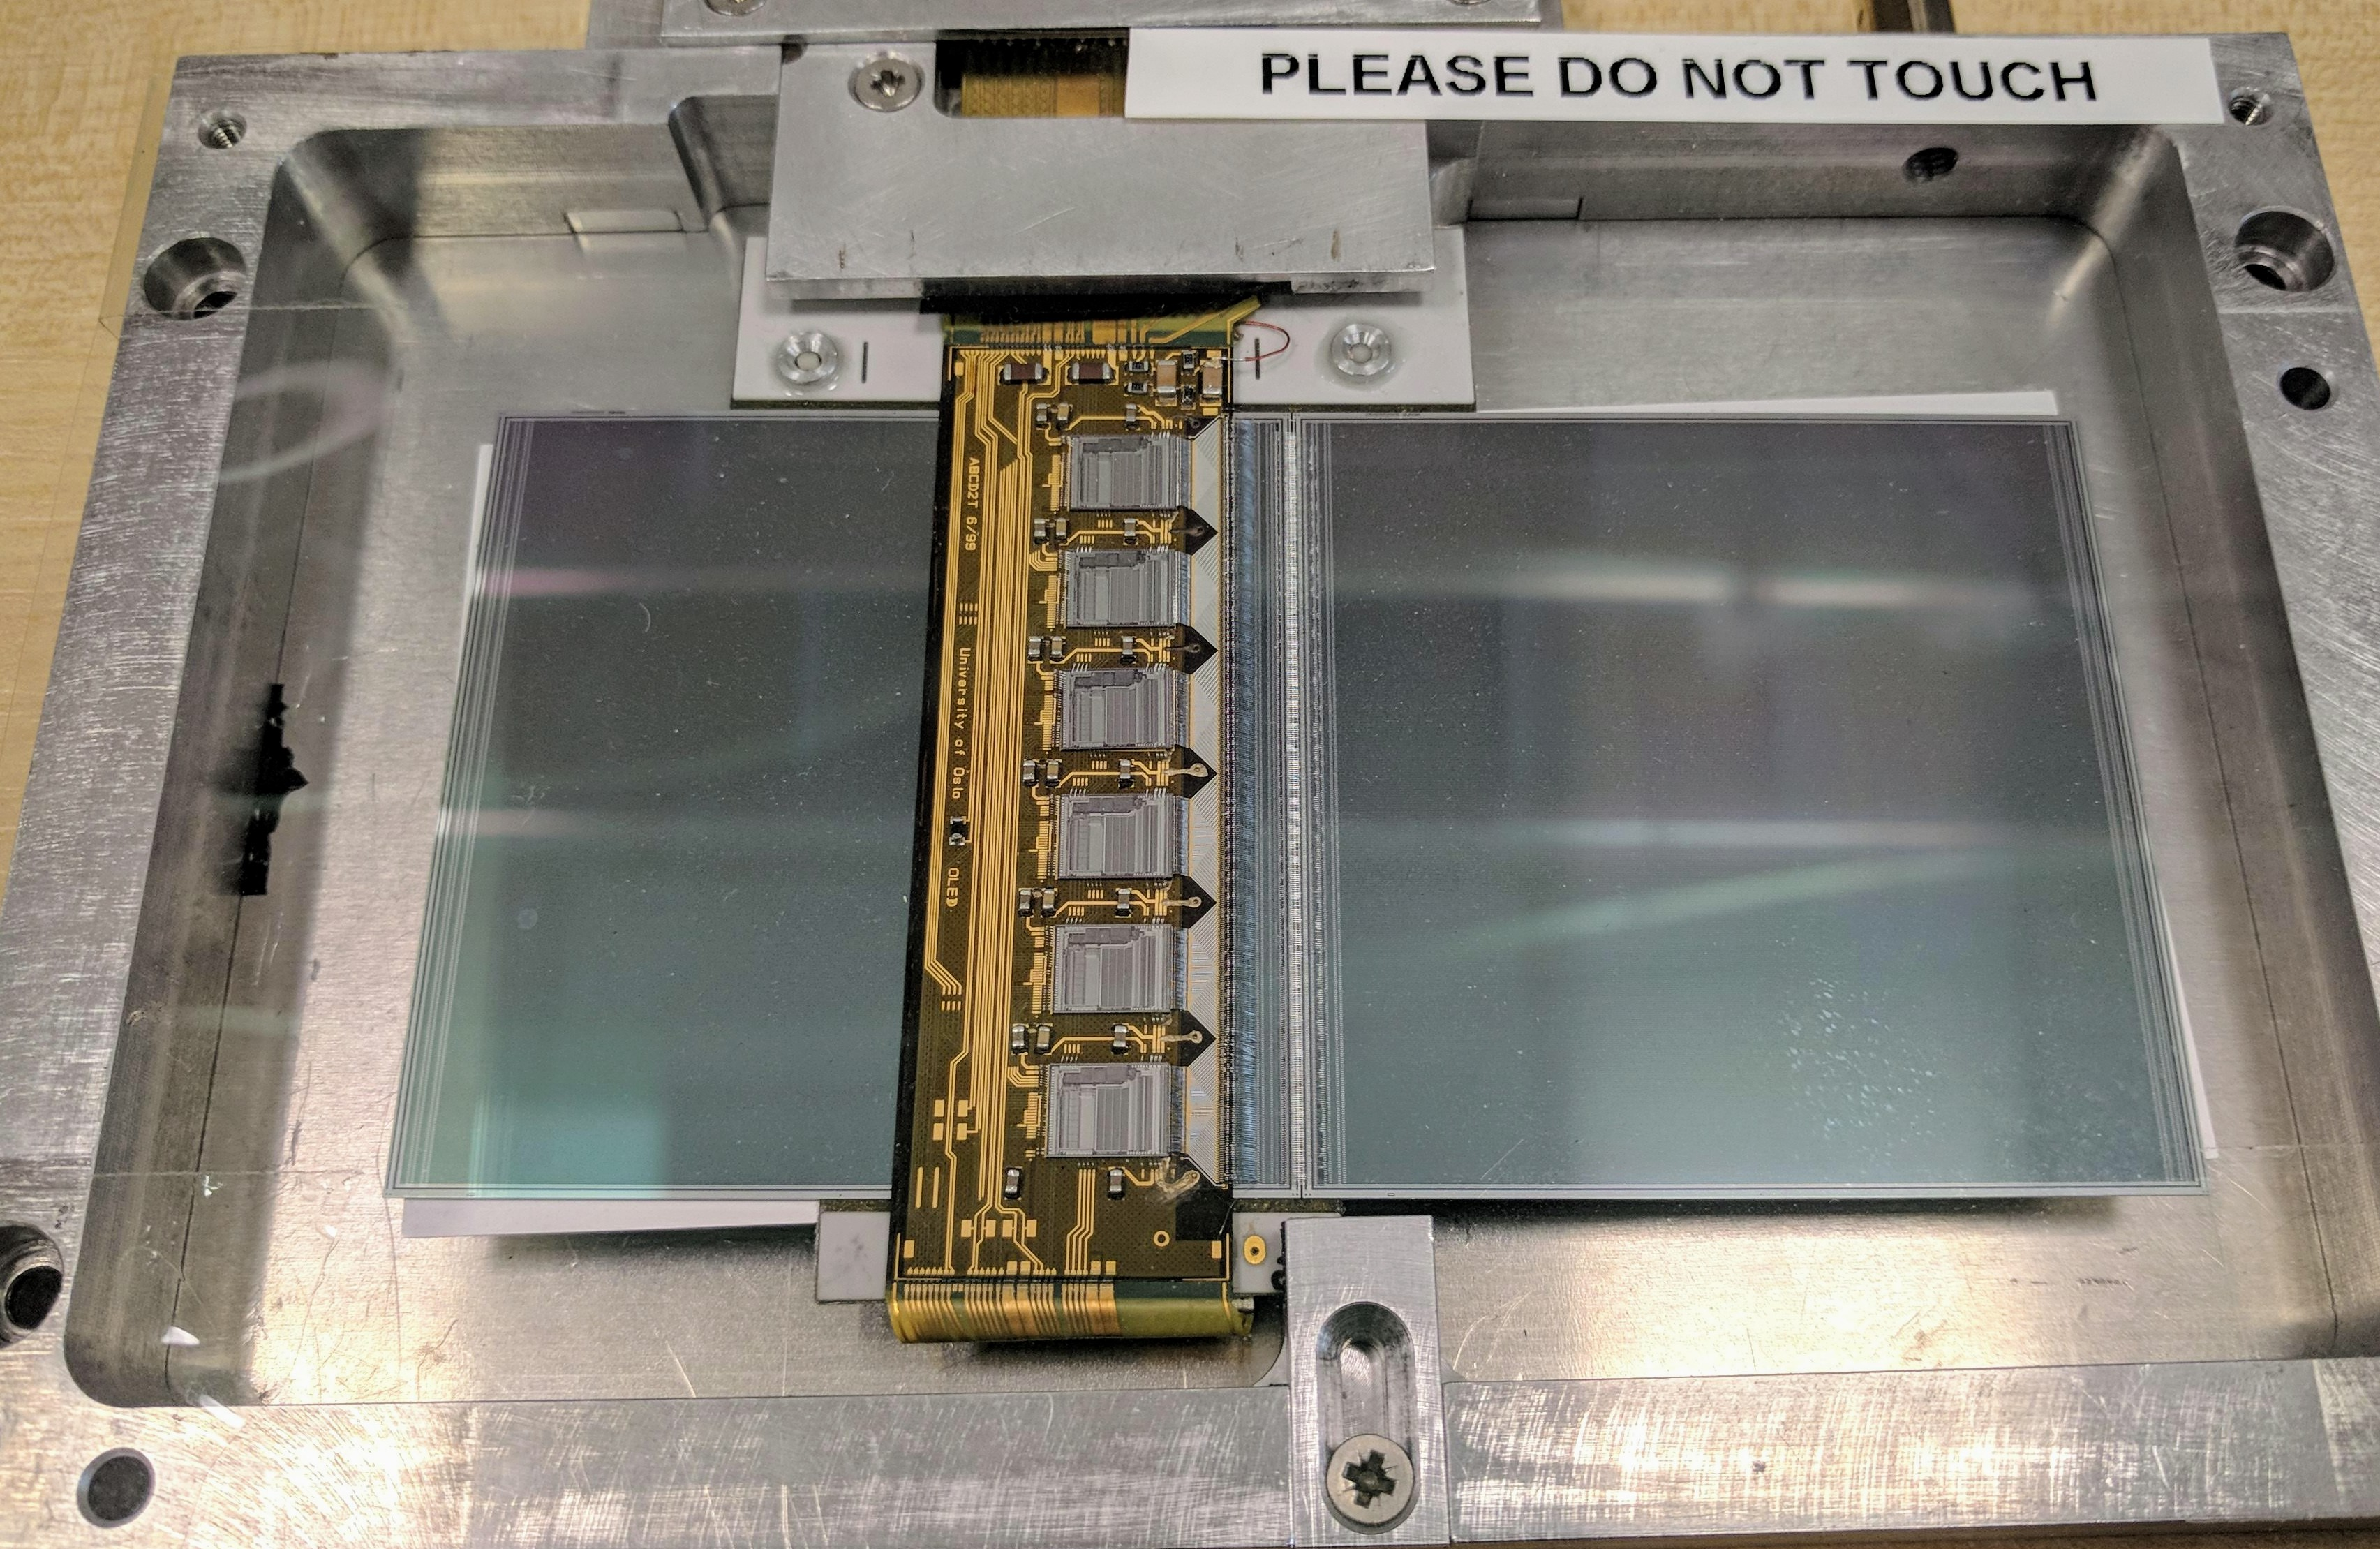
\includegraphics[width=.7\textwidth]{sct-module}
  \caption[ATLAS long strip module]{An image of an SCT long strip module
    mounted in a rig for testing at Queen Mary Univesity of London.}
  \label{fig:strip-module}
\end{figure}
In order to calibrate the response of the strips a 100~M$\Omega$ poly-silicon
resistor is located at the end of each strip. Figure~\ref{fig:sct-close} shows an
image of the snake-like structure of a poly-silicon resistor from the end of an
SCT module.
\begin{figure}[h]
  \centering
  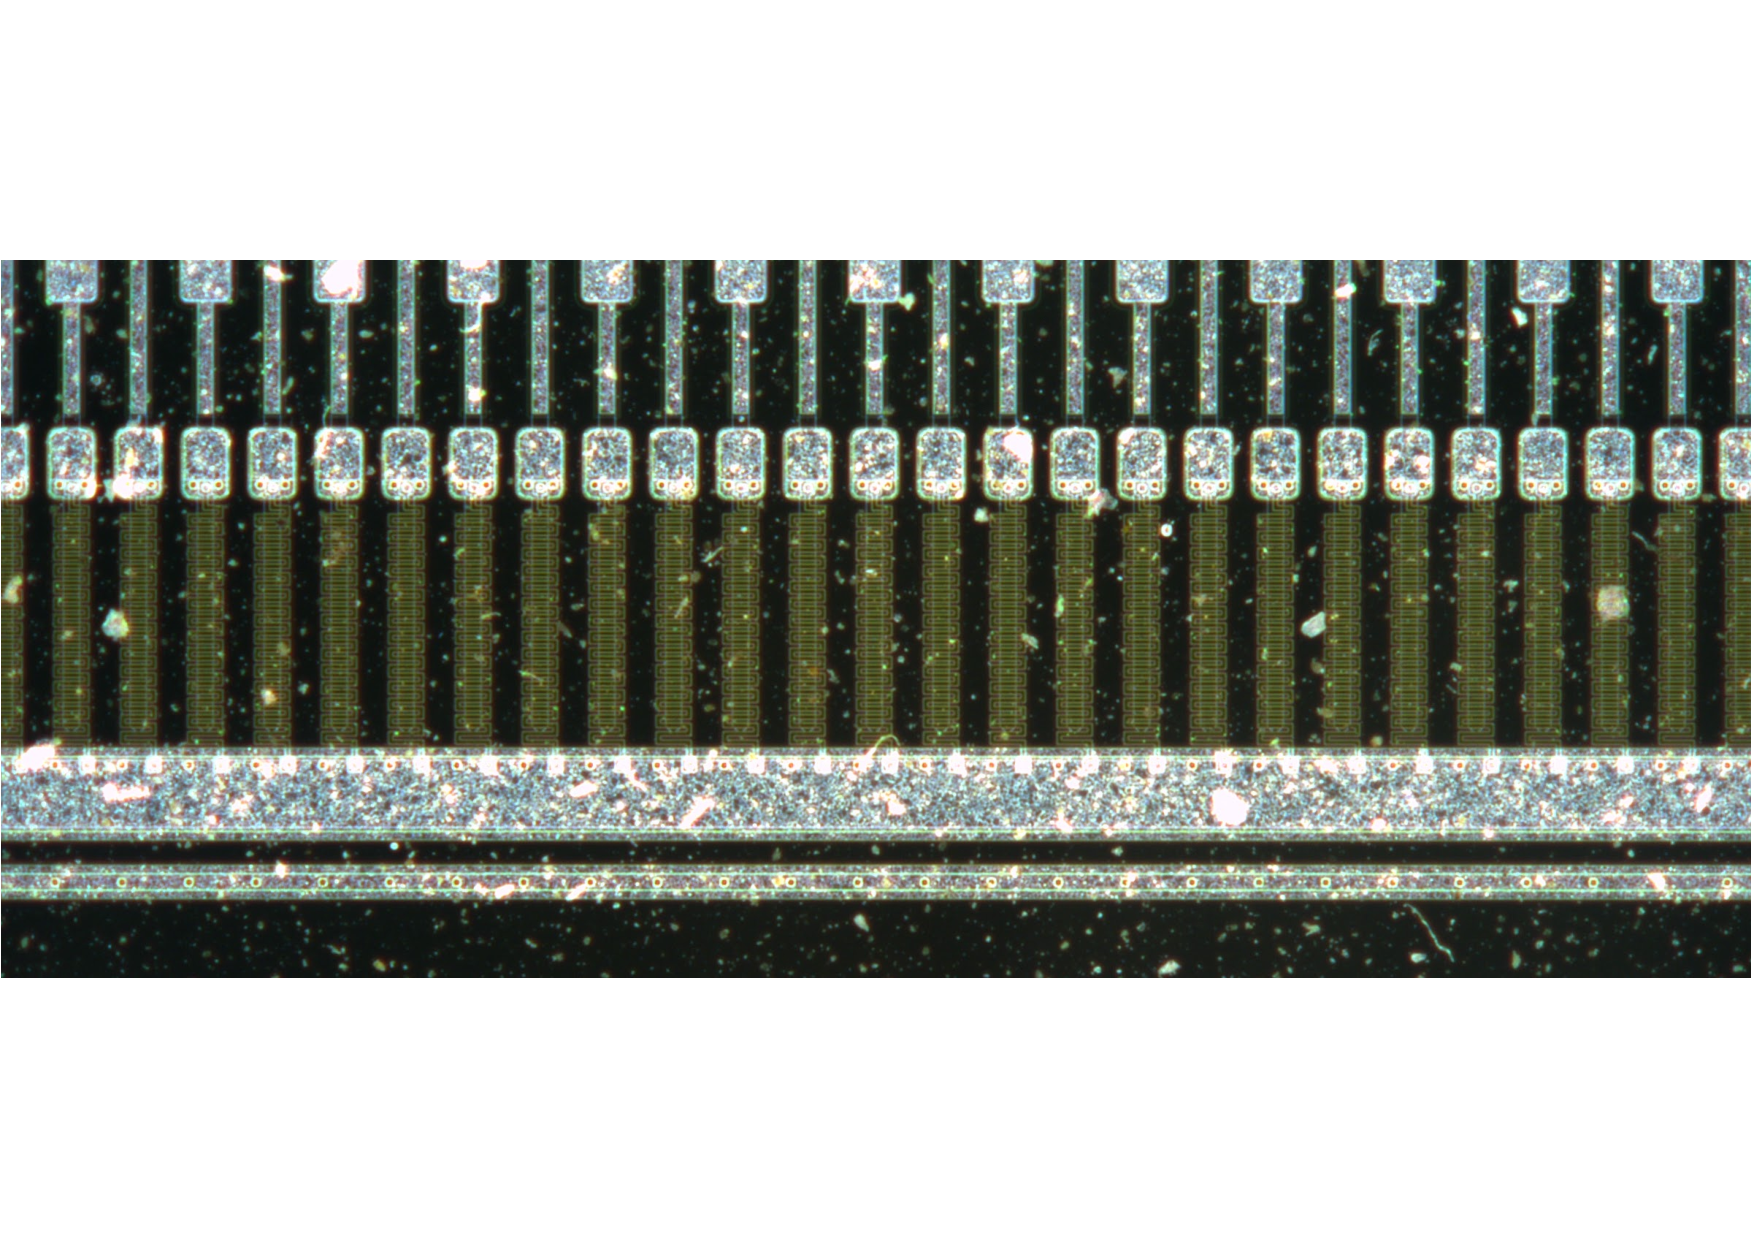
\includegraphics[width=.7\textwidth]{sct-close}
  \caption[ATLAS strip close-up]{A close up image of the end of an SCT sensor in
    which the snake-like poly-silicon reistors are visible as a yellowish
    coloured structure at the end of each strip. This image was taken with a
    high resolution automatic area scanner commissioned by the
    author~\cite{itk-scanner} in order to take full scans of strip sensors
    during the production of the ATLAS Inner Detector upgrade known as the Inner
    Tracker (ITk)~\cite{itk-tdr, itk-strips-tdr}.}
  \label{fig:sct-close}
\end{figure}
The modules come in two different designs, short strips and long
strips with the short strips forming the layer closest to the pixel detectors
and the long strips on the outside.

The original operating bias voltage was 150~V but again due to radiation
exposure this will raise to up to 350~V over time as necessary. There are four
layers of semiconductor trackers in the barrel arranged so that sensors have a
tilt with respect to a perfect coaxial cylinders of approximately 11~$\degree$.
This tilt increases the amount of material that particles will travel through
and is optimized to the geometry of the detector. Similarly the end-cap modules
are arranged in petal like structures, with a number of different geometric
designed based on the position within the end-cap.

\subsubsection{Transition Radiation Tracker}

The final layer of the ID is the TRT, the primary role of the TRT is to aid
electron identification by measurement of transition radiation. The TRT is
mostly made up of polyimide drift tubes with a diameter of 4~mm. The drift tubes
are filled with a gas mixture whose majority constituent is xenon. These tubes
operate with a voltage of -1530~V and are contained within a carbon fibre
support structure. The geometrics layout of the tubes is optimized for
both the barrel and end-caps.

\subsection{Calorimeters}%
\label{sec:calo}

The purpose of the calorimeters is to measure the total energy of particles that
pass all the way through the ID, this is achievable only if the calorimeter
stops the particle completely. A desirable side effect is that they also act as
a barrier to stop particles passing through to the muon spectrometers, of course
this means necessarily that muons pass through the calorimeters. There are two
calorimeter systems in ATLAS the electromagnetic calorimeter (ECAL) and the
hadronic calorimeter (HCAL), they will be explained in the following sections.
The calorimeters are not immersed in a significant magnetic field compared to
the rest of the ATLAS as seen in the heat map of figure~\ref{fig:ATLAS-magnets}.
This is because measuring the energy of

particles and acting as a barrier to them does not require curved trajectories.
The geometric layout of the calorimeter systems, as well as the location of
specific components can be seen in figure~\ref{fig:ATLAS-calo}, in which the ID
can also be seen (greyed out). Information from the two calorimeters is used in
conjunction for any particles whose decay products propagate through both
volumes. Both calorimeters are split up into cells of material that are used to
determine the position of decay products in the detector.
\begin{figure}[h]
  \centering
  \includegraphics[width=.7\textwidth]{ATLAS-calo}
  \caption[ATLAS Calorimeter]{Computer Generated image of the ATLAS
    calorimeter~\cite{ATLAS-calo-fig}.}%
  \label{fig:ATLAS-calo}
\end{figure}

\subsubsection{Electromagnetic Calorimeter}
The ECAL is primarily concerned with measuring the energy and stopping the
trajectory of electrons and photons. It has liquid argon (LAr) as it's active
material. Particles initiate an electromagnetic shower of decay products in the
active material which ionizes it. An applied electric field causes these ions to
drift in such a way that the current induced is proportional to the energy
deposited by the incident particle.

\subsubsection{Hadronic Calorimeter}
The HCAL also has a LAr component which works in a similar way to that of the
ECAL but with different optimizations for the HCAL's specialised design. The
HCAL is specifically tasked with measuring the energy and stopping the
trajectory of hadrons. The HCAL also contains a tile calorimeter which uses
scintillation light produced in the tiles as a means to measure the deposited
energy of hadrons.

\subsection{Muon Spectrometers}%
\label{sec:muon}

Surrounding the calorimeters are the muon spectrometers, which form the most
outer layer of the detector. Though muons are charged leptons just like
electrons, their specific properties mean that dedicated muon spectrometers are
required to detect them. Muons deposit far less energy per distance traveled
than other particles meaning that they punch through most materials with ease.
As can be seen in figure~\ref{fig:ATLAS-muon} the components of the muon
spectrometers are the thin-gap chambers, cathode strip chambers, resistive plate
chambers and monitor drift tubes. The barrel and end-cap toroid magnets immerse
the muon spectrometers in a magnetic field which at its peak (visible in
figure~\ref{fig:ATLAS-magnets}) has a strength of 4~T. Despite a stronger
peaking magnetic field than in the solenoid observed muon tracks are often far
less curved than that of their lighter cousins, the electrons. This is due to the
larger mass of the muon. Muons do leave tracks in the ID and also deposit
small amounts of energy in the calorimeters. Tracks in the muon spectrometers are
matched up to tracks in the ID with the aid of the location of energy deposits
in the calorimeters if possible. The full tracking information for muons can be
used in algorithms such as overlap removal, which is used to remove muons from
jets that they have been erroneously associated with by matching the muon with
its ID track.
\begin{figure}[h]
  \centering
  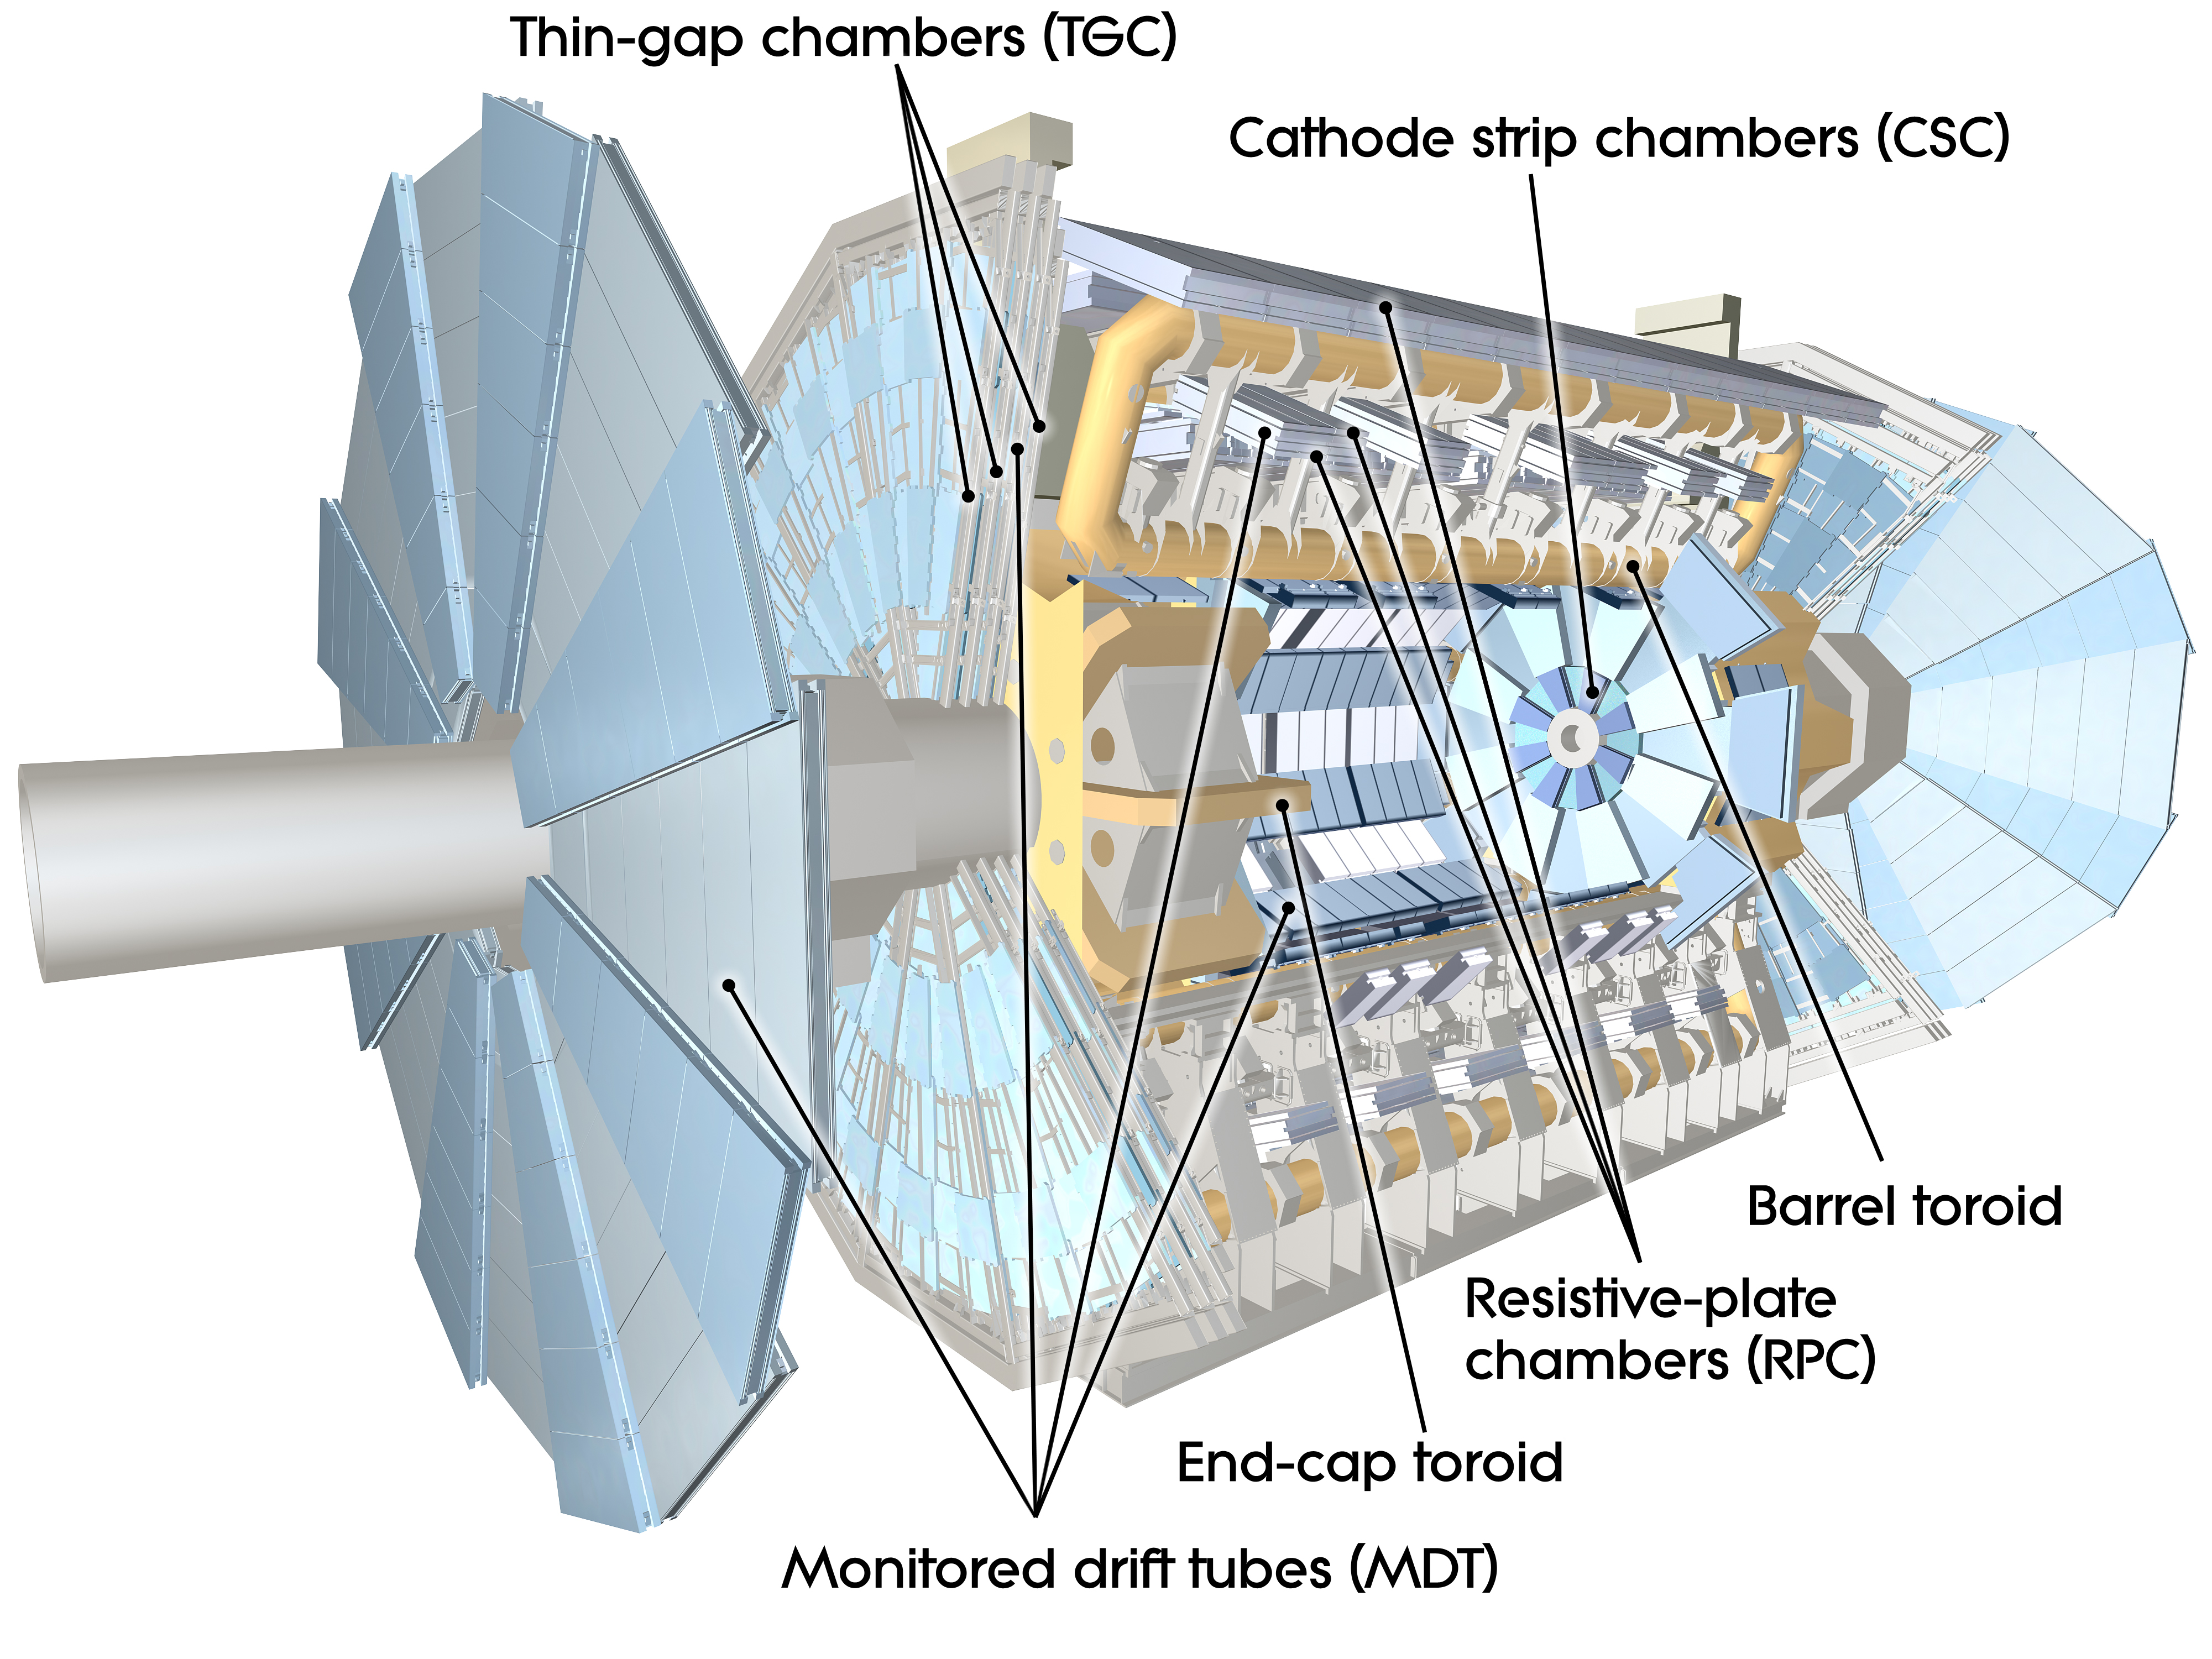
\includegraphics[width=.7\textwidth]{ATLAS-muon-spec}
  \caption[ATLAS muon subsystem]{Computer generated image of the ATLAS Muons
    subsystem~\cite{ATLAS-muon-fig}.}%
  \label{fig:ATLAS-muon}
\end{figure}

\subsection{Trigger Systems}%
\label{sec:trigger}

The trigger systems in ATLAS allows data to be recorded only when an event meets
certain criteria. Without triggering there would be no way to decide which
events to readout and which to ignore. It would be impossible to readout every
interaction that occurs in the detector. The reason for this is that the
geometric constraints of the detector mean that there is only a small space
available for readout wires, as detection medium needs to be prioritized for
sensitivity and technology limits the data rate that one can achieve through a
cable of fixed area. The trigger system comes in two parts, a hardware component
referred to as level one (L1) and software component referred to as the high
level trigger (HLT). The L1 system is comprised of the L1 calorimeter (L1Calo)
trigger which operates by searching for clusters of energy in the calorimeters
and the L1 muon (L1Muon) system which coincidences in the muon systems. A third
system L1 topological (L1Topo) uses regions of interest built from the L1Calo
and L1Muon data which are passed to central trigger processors for selection.
The various limitations of the hardware mean that these selections must be
passed up to the next level of triggering, the HLT in a time window of
2.5~$\mu$s. The HLT takes information from the L1 systems and uses faster
versions of an offline style analysis in order to select or reject events for
readout. In order for a  trigger to fire an event must pass fully all of the
requirements of one of the algorithms defined by an extensive trigger menu. More
information about the triggers used in the $VH(bb)$ analysis will be given in a
later chapter.
